\section{Objectives}
Complete both diode-load CS circuits, the current-source-load CS and N/P source followers from \textit{AIC Lab.pdf}, PDF pages 31--40. Check geometry, bias, output resistance, gain and bandwidth for each case. The model library is supplied separately by the user. The 1.0 V supply is a teaching adaptation, not a certification of the model voltage rating. Numerical plots for the handout's original 3.3 V process are not used directly as pass thresholds. The circuits are rebuilt from the handout topology; the earlier code is used only to review dimensions and omissions.

\section{Specification Mapping}
S denotes actual simulation and D denotes derivation/discussion. The old-process gain tables are background comparisons, not guarantees for the supplied model.
\small\begin{longtable}{p{.46\linewidth}p{.30\linewidth}p{.15\linewidth}}\toprule
Requirement and PDF pages & Deck / check & Status \\ \midrule\endhead
PMOS diode-load CS, W=100/200/300 (31--32) & D01; DC/AC/Rout & S+D \\
NMOS diode-load CS, W=150/200/300 (33--34) & D02; DC/AC/Rout & S+D \\
Diode-load gain, gain-bandwidth and tradeoffs (34) & D01--02; derivatives & S+D \\
Current-load CS, equal-W/L scaling and mirror accuracy (35--37) & D03/C0,C5,C6 & S+D \\
NMOS/PMOS source followers (38--39) & D04; gain/BW & S+D \\
CS W=10/18/26 and Iref=100/166/333 (39--40) & D03/C0--C4 & S+D \\
Low-current adaptation and time-domain check & D03/C7--C9, D05 & S; adapted \\
\bottomrule\end{longtable}\normalsize


\section{Circuit and Design Derivation}
\[
A_{v,P}\simeq-\frac{g_{m1}}{g_{ds1}+g_{m2}+g_{ds2}},\quad
A_{v,N}\simeq-\frac{g_{m1}}{g_{ds1}+g_{m2}+g_{mb2}+g_{ds2}}.
\]
\[
A_{v,CS}\simeq-\frac{g_{mn}}{g_{dsn}+g_{dsp}},\qquad
A_{v,SF}\simeq\frac{g_m}{g_m+g_{mb}+g_{ds,F}+g_{ds,load}}.
\]The derivative estimate uses each case's actual \texttt{.op} values, not an assumed mobility. $R_o$ is obtained from the small-signal \texttt{.tf} output resistance, with capacitors open at DC. $GB=|A_v(1\,\mathrm{Hz})|f_{3dB}$ is stored separately from the actual unity crossing; the two are not forced to agree in a multipole circuit.

D01/D02 retain the handout $W/L=2/1\,\mu$m load and $C_L=10$ pF, sweep the specified input-device widths, and use $L=1\,\mu$m. The page 33 statement tying an NMOS body to VDD is inconsistent with a conventional P-substrate implementation; the body is grounded here and $g_{mb}$ is retained. These two diode-load topologies were absent from the earlier code and are now included.

D03/C0--C4 use $(W_n,W_p,L,I_{ref})=(10,30,1,100)$, $(18,30,1,100)$, $(26,30,1,100)$, $(10,30,1,166)$ and $(10,30,1,333)$, with dimensions in $\mu$m and current in $\mu$A. C5/C6 multiply every W and L of C0 by 3/5, preserving W/L. C7--C9 are explicit 10 $\mu$A adaptations with $W_n=10/18/26\,\mu$m. Each CS input bias is calibrated from its DC transfer and local derivative to approximately 0.5 V output; no servo amplifier is added to the device under test.

D04 uses $W/L=30/1\,\mu$m and $C_L=10$ pF for both followers, with NMOS/PMOS gate biases of 0.9/0.1 V. C0--C3 use 100/10/166/333 $\mu$A. Consistent circuits across analyses replace the earlier mismatched DC/AC/transient dimensions and beyond-rail input signals.

\section{Simulation Setup}
Runs use PrimeSim HSPICE S-2021.09 win64, a baseline temperature of 27 $^\circ$C, \texttt{runlvl=5}, \texttt{accurate}, and \texttt{.op/.print/.measure} outputs. Every \texttt{.alter} resets all baseline parameters and temperature to prevent state from carrying into the next case. Actual runs completed without an error or failed measurement. Suppressed model warnings remain, so a warning-free run is not claimed. Public netlists contain no model paths. This comment marks the model setup required locally before execution; the model and its configuration remain local:
\begin{verbatim}
* MODEL_SETUP_REQUIRED
\end{verbatim}
CSV files and numerical summaries are in the lab's \texttt{results/} directory. Every figure is redrawn from actual printed data, not a waveform-viewer screenshot. \texttt{manifest.json} supplies specification mapping and case definitions.Five decks contain 23 cases. CS DC sweeps use 0--1 V in 1 mV steps; AC uses 1 Hz--10 GHz, 60 points/decade and a 1 V input. The follower DC sweep changes only the NMOS input; PMOS stays at 0.1 V. Its N/P AC circuits are independent, avoiding normalization against oppositely phased inputs. D05 runs a 1 kHz signal for 5 ms and measures peak-to-peak output over the last period. CS amplitudes are 0.1/1/3 mV; follower amplitude is 10 mV.

\section{Results and Specification Checks}
\begin{center}\small\begin{tabular}{lrrrrrr}\toprule
Case & $V_{in}$ (V) & $|A_v|$ & $g_m$ estimate & $R_o$ (k$\Omega$) & $f_{3dB}$ (MHz) & Sat. \\ \midrule
D01/C0 & 0.21622 & 2.35 & 2.35 & 43.07 & 0.366 & Y \\
D01/C1 & 0.18785 & 2.41 & 2.41 & 43.05 & 0.363 & Y \\
D01/C2 & 0.17159 & 2.44 & 2.45 & 43.04 & 0.360 & Y \\
D02/C0 & 0.19697 & 1.11 & 1.11 & 21.35 & 0.736 & Y \\
D02/C1 & 0.18532 & 1.13 & 1.13 & 21.35 & 0.733 & Y \\
D02/C2 & 0.16909 & 1.14 & 1.14 & 21.35 & 0.727 & Y \\
D03/C0 & 0.55243 & 124.30 & 124.34 & 126.10 & 0.125 & Y \\
D03/C1 & 0.49981 & 156.65 & 156.69 & 125.30 & 0.126 & Y \\
D03/C2 & 0.47225 & 174.09 & 174.13 & 123.60 & 0.128 & Y \\
D03/C3 & 0.60983 & 69.37 & 69.39 & 54.73 & 0.289 & Y \\
D03/C4 & 0.71517 & 11.10 & 11.10 & 6.68 & 2.363 & N \\
D03/C5 & 0.55481 & 179.14 & 179.92 & 181.20 & 0.086 & Y \\
D03/C6 & 0.55539 & 201.82 & 204.63 & 204.10 & 0.075 & Y \\
D03/C7 & 0.39126 & 227.10 & 227.14 & 1208.00 & 0.013 & Y \\
D03/C8 & 0.36092 & 233.00 & 233.05 & 1159.00 & 0.014 & Y \\
D03/C9 & 0.34283 & 234.85 & 234.92 & 1133.00 & 0.014 & Y \\
\bottomrule\end{tabular}\end{center}
Sat.=Y only means that every device at this nominal operating point satisfies $|V_{DS}|\ge|V_{DSAT}|$. It does not imply strong inversion or valid operation across the entire output swing. Subthreshold labels remain in \texttt{operating\_points.csv}. The diode-load CS devices often enter weak inversion under these biases, so the strong-inversion $\sqrt W$ gain scaling must not be imposed.

\begin{figure}[htbp]\centering
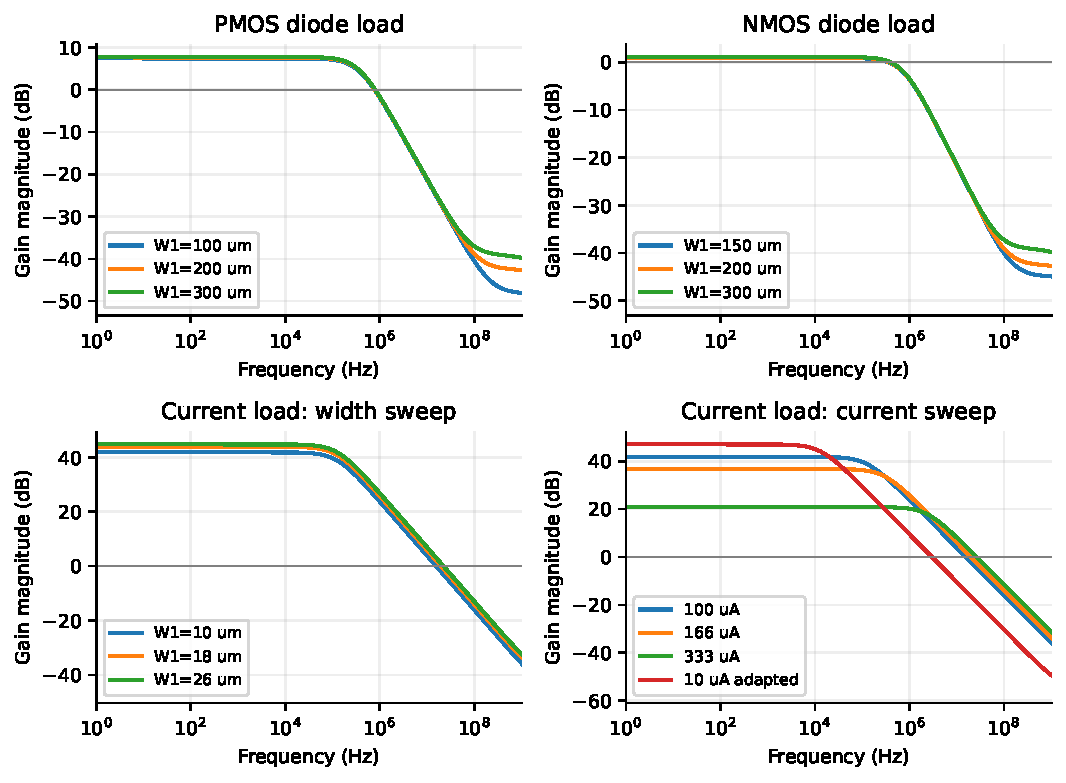
\includegraphics[width=\linewidth]{figures/gain_comparison.pdf}
\caption{Actual Bode curves for both diode loads and current-source loads. Each geometry/current comparison retains its own operating point.}
\end{figure}
\begin{center}\small\begin{tabular}{lrrrr}\toprule
$I_{ref}$ ($\mu$A) & $A_n$ & $A_p$ & $f_n$ (MHz) & $f_p$ (MHz) \\ \midrule
100 & 0.8260 & 0.6855 & 27.032 & 12.355 \\
10 & 0.8337 & 0.8503 & 3.992 & 2.856 \\
166 & 0.8217 & 0.5344 & 38.088 & 17.654 \\
333 & 0.8079 & 0.4060 & 57.736 & 25.284 \\
\bottomrule\end{tabular}\end{center}
\begin{center}\small\begin{tabular}{lrrr}\toprule
Input amplitude (mV) & CS output p-p (V) & Effective $|A_v|$ & Follower p-p (V) \\ \midrule
0.1 & 0.04521 & 226.04 & 0.01667 \\
1 & 0.42794 & 213.97 & 0.01667 \\
3 & 0.74588 & 124.31 & 0.01667 \\
\bottomrule\end{tabular}\end{center}
\begin{center}\small\begin{tabular}{lrr}\toprule
D03 case & Mirror error (\%) & $GB$ (MHz) \\ \midrule
0 & -0.492 & 15.594 \\
1 & -0.492 & 19.764 \\
2 & -0.492 & 22.256 \\
3 & -0.968 & 20.051 \\
4 & -3.926 & 26.230 \\
5 & -0.337 & 15.450 \\
6 & -0.292 & 15.224 \\
7 & 0.392 & 2.976 \\
8 & 0.392 & 3.180 \\
9 & 0.392 & 3.278 \\
\bottomrule\end{tabular}\end{center}
D03 mirror error is $(|I_{MP}|/|I_{MREF}|-1)\times100\%$. The 333 $\mu$A case is retained, but reduced reference headroom and device operating regions limit its gain; width alone does not explain the result. D05 with 0.1 mV input approaches the small-signal response. Larger amplitudes reduce effective gain because of DC-transfer curvature.
\begin{figure}[htbp]\centering
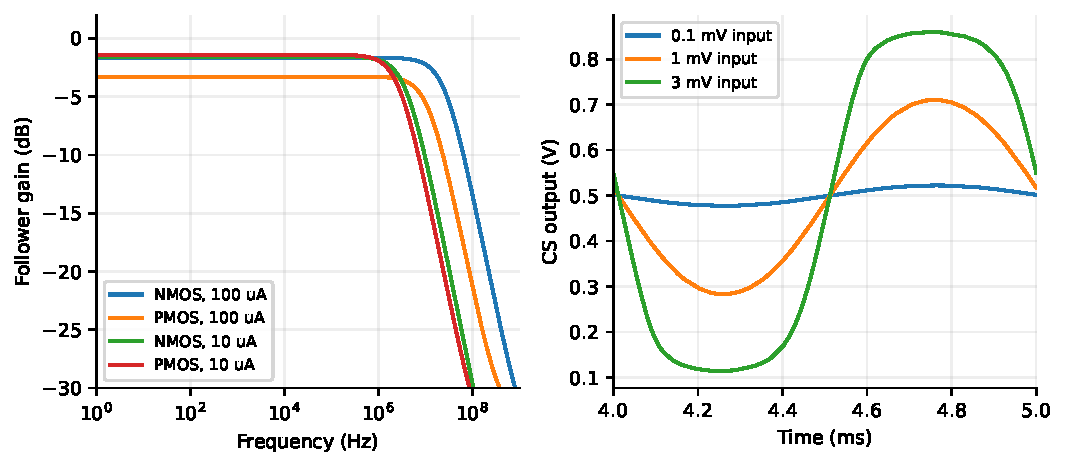
\includegraphics[width=\linewidth]{figures/followers_transient.pdf}
\caption{N/P follower frequency responses and the CS amplitude comparison. The right panel shows actual output during the final 1 kHz period.}
\end{figure}


\section{Discussion}
For equal load geometry, mobility, bias and the absence of the same NMOS source-body term can give the PMOS diode load a smaller load transconductance and greater CS gain. This is conditional, not universal across processes and biases. Diode loads are simple to bias, use few devices and give low output resistance, at the expense of gain and voltage headroom. Increasing input $g_m$ or reducing effective load admittance can raise gain; more current or less load capacitance can improve speed while also changing power, output resistance and bias.

A current-source load removes the load $g_m$ term, increasing gain but making the output bias more sensitive to current matching. At fixed current, larger W can increase strong-inversion $g_m$ while also adding capacitance. Increasing current changes both $g_m$ and $g_{ds}$ and need not increase gain. Longer L at equal W/L can reduce channel-length modulation and improve mirror accuracy, but costs area and parasitic capacitance.

Body effect and finite load conductance reduce source-follower gain. NMOS is closer to unity at 100 $\mu$A, but at 10 $\mu$A this PMOS result is approximately 0.8503, higher than NMOS at approximately 0.8337. The N-type advantage in the old plot is not a universal rule.

\section{Conclusion}
The specified topologies and width, current and equal-W/L scale variations have been simulated, including the previously missing diode loads. Gain, bandwidth and nonlinear results apply to their declared biases. Old-process numerical agreement and full-PVT success are not claimed.

